% vim: set spell spelllang=en tw=100 et sw=4 sts=4 foldmethod=marker foldmarker={{{,}}} :

\documentclass{beamer}

\usepackage{tikz}
\usepackage{xcolor}
\usepackage{complexity}
\usepackage{hyperref}
\usepackage{microtype}
\usepackage{amsmath}                   % \operatorname
\usepackage{amsfonts}                  % \mathcal
\usepackage{amssymb}                   % \nexists
\usepackage{gnuplot-lua-tikz}          % graphs
\usepackage[vlined]{algorithm2e} % algorithms
\usepackage{centernot}
\usepackage{mathtools}
\usepackage{listings}

\usetikzlibrary{shapes, arrows, shadows, calc, positioning, fit}
\usetikzlibrary{decorations.pathreplacing, decorations.pathmorphing, shapes.misc}
\usetikzlibrary{tikzmark}

\definecolor{uofguniversityblue}{rgb}{0, 0.219608, 0.396078}

\definecolor{uofgheather}{rgb}{0.356863, 0.32549, 0.490196}
\definecolor{uofgaquamarine}{rgb}{0.603922, 0.72549, 0.678431}
\definecolor{uofgslate}{rgb}{0.309804, 0.34902, 0.380392}
\definecolor{uofgrose}{rgb}{0.823529, 0.470588, 0.709804}
\definecolor{uofgmocha}{rgb}{0.709804, 0.564706, 0.47451}
\definecolor{uofgsandstone}{rgb}{0.321569, 0.278431, 0.231373}
\definecolor{uofgforest}{rgb}{0, 0.2, 0.129412}
\definecolor{uofglawn}{rgb}{0.517647, 0.741176, 0}
\definecolor{uofgcobalt}{rgb}{0, 0.615686, 0.92549}
\definecolor{uofgturquoise}{rgb}{0, 0.709804, 0.819608}
\definecolor{uofgsunshine}{rgb}{1.0, 0.862745, 0.211765}
\definecolor{uofgpumpkin}{rgb}{1.0, 0.72549, 0.282353}
\definecolor{uofgthistle}{rgb}{0.584314, 0.070588, 0.447059}
\definecolor{uofgrust}{rgb}{0.603922, 0.227451, 0.023529}
\definecolor{uofgburgundy}{rgb}{0.490196, 0.133333, 0.223529}
\definecolor{uofgpillarbox}{rgb}{0.701961, 0.047059, 0}
\definecolor{uofglavendar}{rgb}{0.356863, 0.301961, 0.580392}

\tikzset{vertex/.style={draw, circle, inner sep=0pt, minimum size=0.5cm, font=\small\bfseries}}
\tikzset{notvertex/.style={vertex, color=white, text=black}}
\tikzset{plainvertex/.style={vertex}}
\tikzset{vertexc1/.style={vertex, fill=uofgburgundy, text=white}}
\tikzset{vertexc2/.style={vertex, fill=uofgsandstone, text=white}}
\tikzset{vertexc3/.style={vertex, fill=uofgforest, text=white}}
\tikzset{vertexc4/.style={vertex, fill=uofgheather, text=white}}
\tikzset{edge/.style={color=black!50!white}}
\tikzset{bedge/.style={ultra thick}}
\tikzset{edged/.style={color=screengrey, dashed}}
\tikzset{edgel3/.style={color=uofgrose, ultra thick}}

% {{{ theme things
\useoutertheme[footline=authortitle]{miniframes}
\useinnertheme{rectangles}

\setbeamerfont{block title}{size={}}
\setbeamerfont{title}{size=\large,series=\bfseries}
\setbeamerfont{section title}{size=\large,series=\mdseries}
\setbeamerfont{author}{size=\normalsize,series=\mdseries}
\setbeamercolor*{structure}{fg=uofguniversityblue}
\setbeamercolor*{palette primary}{use=structure,fg=black,bg=white}
\setbeamercolor*{palette secondary}{use=structure,fg=white,bg=uofgcobalt}
\setbeamercolor*{palette tertiary}{use=structure,fg=white,bg=uofguniversityblue}
\setbeamercolor*{palette quaternary}{fg=white,bg=black}

\setbeamercolor*{titlelike}{parent=palette primary}

\beamertemplatenavigationsymbolsempty

\setbeamertemplate{title page}
{
    \begin{tikzpicture}[remember picture, overlay]
        \node at (current page.north west) {
            \begin{tikzpicture}[remember picture, overlay]
                \fill [fill=uofguniversityblue, anchor=north west] (0, 0) rectangle (\paperwidth, -2.6cm);
            \end{tikzpicture}
        };

        \node (logo) [anchor=north east, shift={(-0.6cm,-0.6cm)}] at (current page.north east) {
            
\includegraphics[keepaspectratio=true,scale=0.7]{UoG_keyline.pdf}
        };

        \node [anchor=west, xshift=0.2cm] at (current page.west |- logo.west) {
            \begin{minipage}{0.65\paperwidth}\raggedright
                {\usebeamerfont{title}\usebeamercolor[white]{}\inserttitle}\\[0.1cm]
                {\usebeamerfont{author}\usebeamercolor[white]{}\insertauthor}
            \end{minipage}
        };
    \end{tikzpicture}
}

\setbeamertemplate{section page}
{
    \begin{centering}
        \begin{beamercolorbox}[sep=12pt,center]{part title}
            \usebeamerfont{section title}\insertsection\par
        \end{beamercolorbox}
    \end{centering}
}

\newcommand{\frameofframes}{/}
\newcommand{\setframeofframes}[1]{\renewcommand{\frameofframes}{#1}}

\makeatletter
\setbeamertemplate{footline}
{%
    \begin{beamercolorbox}[colsep=1.5pt]{upper separation line foot}
    \end{beamercolorbox}
    \begin{beamercolorbox}[ht=2.5ex,dp=1.125ex,%
        leftskip=.3cm,rightskip=.3cm plus1fil]{author in head/foot}%
        \leavevmode{\usebeamerfont{author in head/foot}\insertshortauthor}%
        \hfill%
        {\usebeamerfont{institute in head/foot}\usebeamercolor[fg]{institute in head/foot}\insertshortinstitute}%
    \end{beamercolorbox}%
    \begin{beamercolorbox}[ht=2.5ex,dp=1.125ex,%
        leftskip=.3cm,rightskip=.3cm plus1fil]{title in head/foot}%
        {\usebeamerfont{title in head/foot}\insertshorttitle}%
        \hfill%
        {\usebeamerfont{frame number}\usebeamercolor[fg]{frame number}\insertframenumber~\frameofframes~\inserttotalframenumber}
    \end{beamercolorbox}%
    \begin{beamercolorbox}[colsep=1.5pt]{lower separation line foot}
    \end{beamercolorbox}
}

% }}}

\title{Table Constraints}
\author{Ciaran McCreesh}

\begin{document}

{
    \usebackgroundtemplate{
        \tikz[overlay, remember picture]
        \node[at=(current page.south), anchor=south, inner sep=0pt]{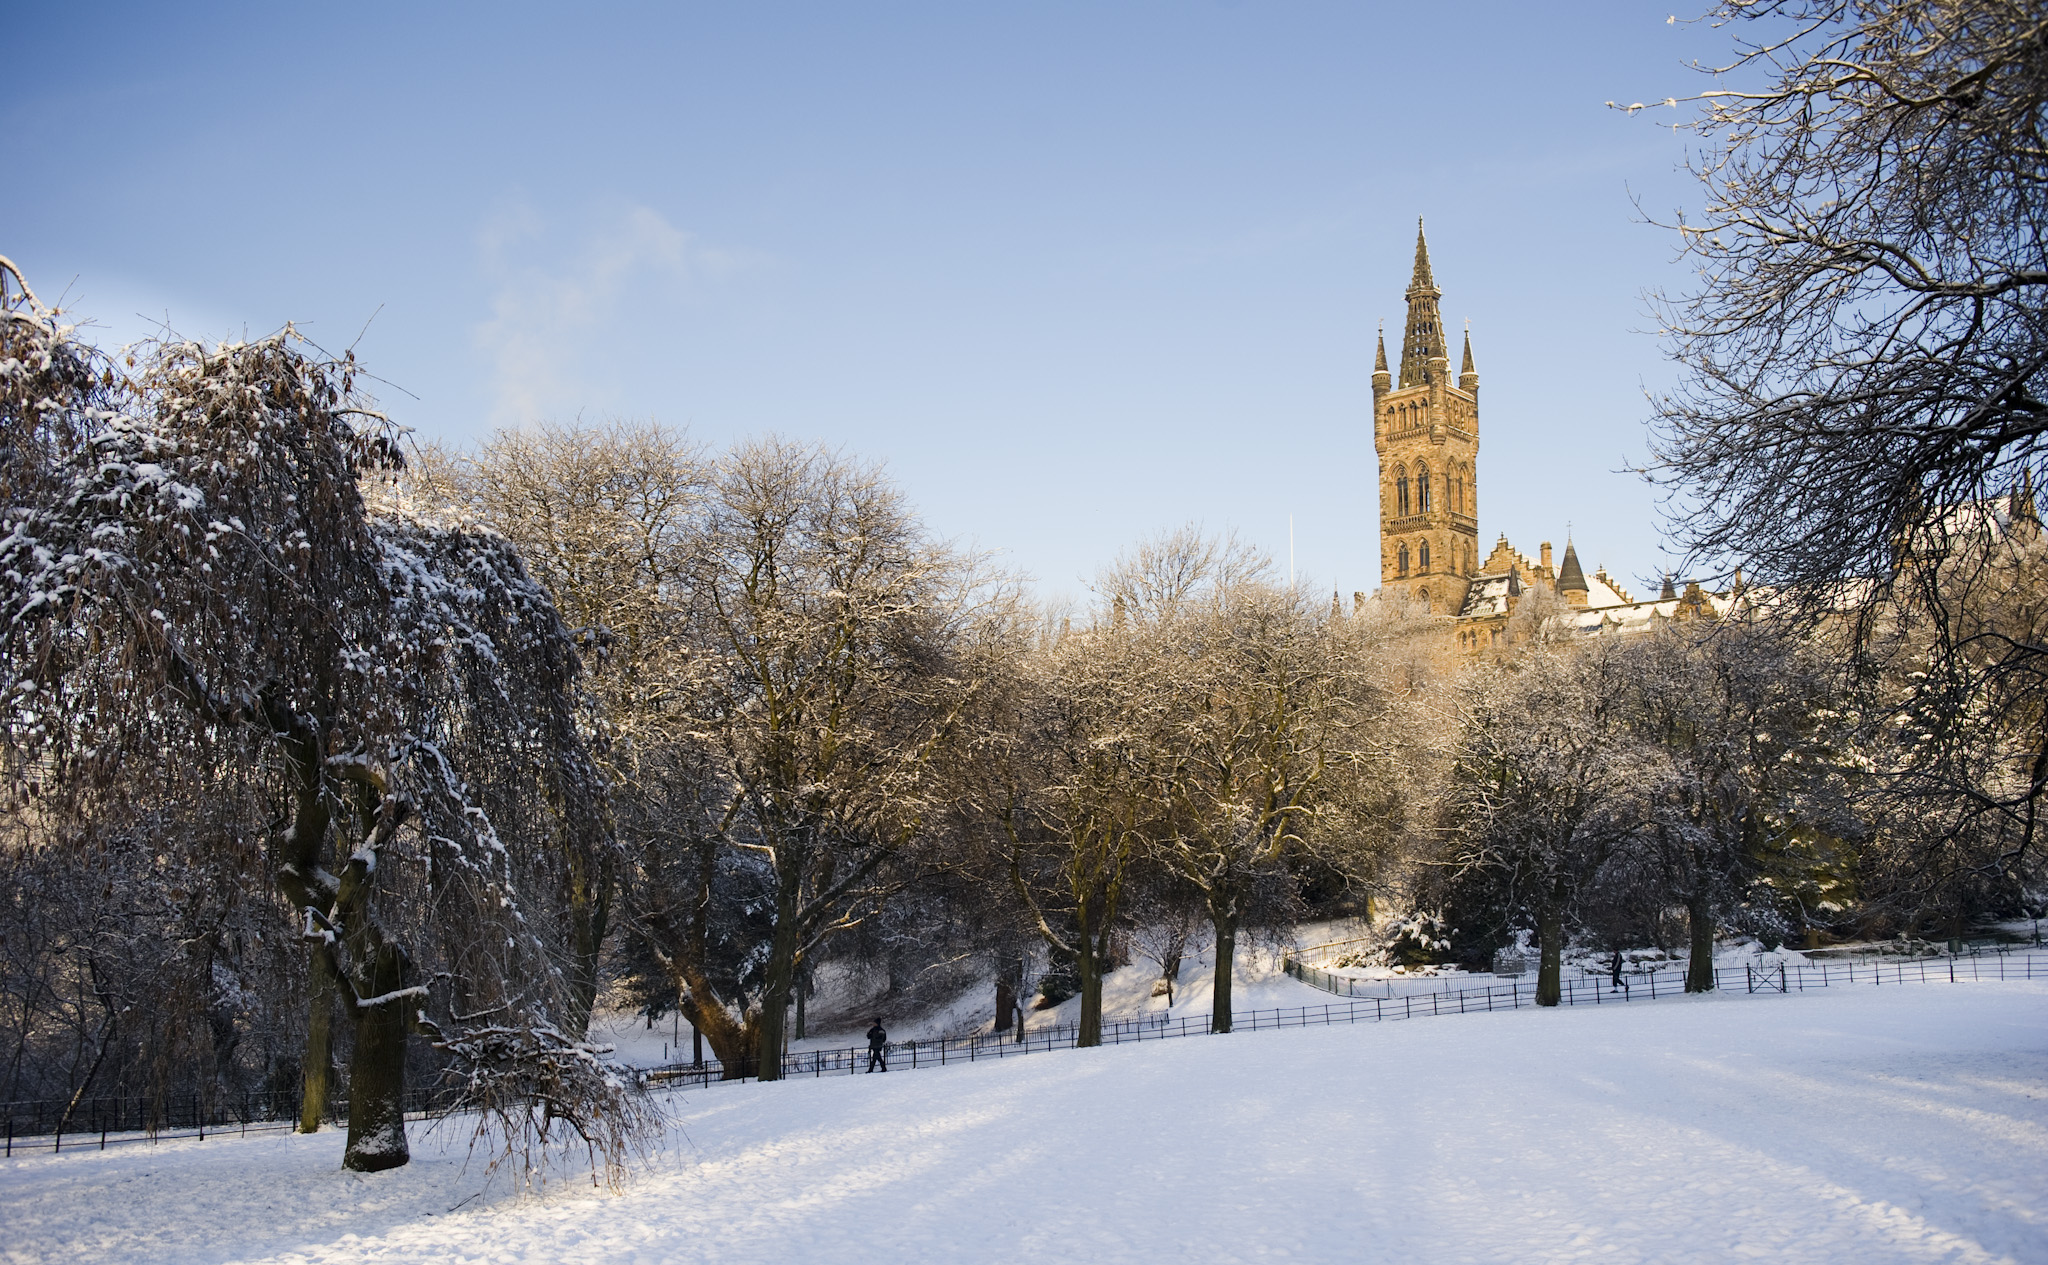
\includegraphics[keepaspectratio=true, width=\paperwidth]{background2.jpg}};
    }
    \begin{frame}[plain,noframenumbering]
        \titlepage
    \end{frame}
}

\begin{frame}{Table Constraints}
    \begin{itemize}
        \item We can represent a constraint as a list of permitted
            tuples: \[ [A, B, C] \in \{ [1, 2, 3], [1, 3, 2], [2, 1, 3], [2, 3,
            1], [3, 1, 2], [3, 2, 1] \} \]
        \item This is the preferred definition for theoretical computer
            science, but not commonly used in practice.
        \item Sometimes table constraints \emph{are} the best option, though.
    \end{itemize}
\end{frame}

\begin{frame}{Consistency, Round Three}
    \begin{itemize}
        \item Back to generalised arc consistency!
        \item Call a tuple \emph{feasible} if each of its values remains in the
            domain of its respective variable.
        \item If each value in each variable is present in at least one
            feasible tuple, we have GAC.
    \end{itemize}
\end{frame}

\begin{frame}{Propagating Table Constraints}
    \begin{itemize}
        \item Keep track of remaining feasible tuples.
        \item For example, by using an additional ``variable'', \begin{align*}
                T = 1 \rightarrow{} &(A = 1 \land B = 2 \land C = 3) \\
                T = 2 \rightarrow{} &(A = 1 \land B = 1 \land C = 2) \\
                T = 3 \rightarrow{} &(A = 2 \land B = 1 \land C = 3) \\
                T = 4 \rightarrow{} &(A = 2 \land B = 3 \land C = 1) \\
                T = 5 \rightarrow{} &(A = 3 \land B = 1 \land C = 2) \\
                T = 6 \rightarrow{} &(A = 3 \land B = 2 \land C = 1)
        \end{align*}
        \item Remove any value that is not supported in a feasible tuple.
    \end{itemize}
\end{frame}

\begin{frame}{Actual Real Constraint Solver Code}
    \vspace*{-0.5em}%
    \only<1>{\lstinputlisting[language=C++, basicstyle=\tiny\ttfamily, keywordstyle=\color{uofgcobalt}]{code/table1.cc}}%
    \only<2>{\lstinputlisting[language=C++, basicstyle=\tiny\ttfamily, keywordstyle=\color{uofgcobalt}]{code/table2.cc}}
\end{frame}

\begin{frame}{Why Not Just Use Table Constraints?}
    \begin{itemize}
        \item We can propagate table constraints in (low) polynomial time, and get GAC.
            \begin{itemize}
                \item There are much faster algorithms than the one on the
                    previous slide.
                \item See: one of the suggested poster papers.
            \end{itemize}
        \item Why not use table constraints for everything?
        \item <2-> Tables can be exponentially long, e.g. for all-different.
    \end{itemize}
\end{frame}

\begin{frame}{Autotabulation}
    \begin{itemize}
        \item Remember Choco being clever with linear equalities?
        \item A solver can turn one or more constraints into a table constraint
            to get more powerful propagation.
        \item If you know when to do this, it can be really powerful.
        \item See: one of the suggested poster papers.
    \end{itemize}
\end{frame}

\begin{frame}{Beyond Table Constraints}
    \begin{itemize}
        \item Smart tables: wildcards, negations, and ranges.
            \begin{itemize}
                \item Can make tables much smaller for some problems.
            \end{itemize}
        \item Decision diagrams.
            \begin{itemize}
                \item Even more compact representations.
            \end{itemize}
        \item Regular expressions.
            \begin{itemize}
                \item See: one of the suggested poster papers.
            \end{itemize}
    \end{itemize}
\end{frame}

\begin{frame}{Shift Pattern Scheduling}
    \vspace*{-0.5em}%
    \only<1>{
        \begin{itemize}
            \item Produce a schedule for eleven employees for two weeks.
            \item Each employee can be on day shift, night shift, or off.
            \item Four employees present on each day shift.
            \item Two employees present on each night shift.
            \item Can't work more than five day shifts in a row.
            \item Can't work more than two night shifts in a row.
            \item Day shift can only be followed by a day shift or a day off.
            \item Night shift can only be followed by a night shift or a day off.
        \end{itemize}
    }%
    \only<2>{\lstinputlisting[basicstyle=\tiny\ttfamily]{code/yaycapitalism1.mzn}}%
    \only<3>{\lstinputlisting[basicstyle=\tiny\ttfamily]{code/yaycapitalism1-out.txt}}%
    \only<4>{\lstinputlisting[basicstyle=\tiny\ttfamily]{code/yaycapitalism2.mzn}}%
    \only<5>{\lstinputlisting[basicstyle=\tiny\ttfamily]{code/yaycapitalism2-out.txt}}%
\end{frame}

\begin{frame}{Ethical Considerations}
    \begin{itemize}
        \item Easy to write a model that produces a valid schedule.
        \item Hard to write a \emph{good} model that doesn't ruin people's lives.
            \begin{itemize}
                \item \emph{Balance} constraints for minimum and maximum hours.
                \item Optimise to respect employee preferences.
            \end{itemize}
        \item <2-> Ethical obligation to support our democratically elected
            capitalist government by maximising shareholder value?
            \begin{itemize}
                \item <2-> Give fewest hours to most expensive employees?
                \item <2-> No need to lay anyone off, just use zero hour contracts?
                \item <2-> Get rid of poorly performing employees by giving them
                    bad shift patterns?
            \end{itemize}
    \end{itemize}
\end{frame}

\begin{frame}[plain,noframenumbering]
    \begin{tikzpicture}[remember picture, overlay]
        \node at (current page.north west) {
            \begin{tikzpicture}[remember picture, overlay]
                \fill [fill=uofguniversityblue, anchor=north west] (0, 0) rectangle (\paperwidth, -1.7cm);
            \end{tikzpicture}
        };

        \node (logo) [anchor=north east, shift={(-0.3cm,-0.2cm)}] at (current page.north east) {
            
\includegraphics[keepaspectratio=true,scale=0.55]{UoG_keyline.pdf}
        };
    \end{tikzpicture}
\end{frame}

\end{document}
